\documentclass[12pt,a4paper,twoside,titlepage,headsepline,numbers=noenddot,listof=totoc,index=totoc,bibliography=totoc]{scrartcl}


\ifx\pdfoutput\undefined
\pdffalse % we are not running pdflatex
\else
\pdfoutput=1 % we are running pdflatex
\pdfcompresslevel=9     % compression level for text and image;
\usepackage[pdftex,bookmarks=true,bookmarksopen=false,bookmarksnumbered=true,linktocpage,colorlinks=true,backref,pagebackref, linkcolor=black,  citecolor=black, urlcolor=black]{hyperref}
\usepackage[pdftex]{graphicx}
\usepackage{microtype}
\fi

\usepackage{amsfonts}
\usepackage{algorithmic}
\usepackage{url}
\usepackage{color}
\usepackage{tabularx}
\usepackage[T1]{fontenc}
\usepackage[utf8x]{inputenc}
\usepackage{textcomp}
\usepackage{bbm}
\usepackage{marvosym}
\usepackage{amsmath}
\usepackage{amssymb}
\usepackage{ntheorem}
\usepackage{fancyvrb}
\usepackage{subfigure}
\usepackage{mathptmx} 
\usepackage[scaled=.90]{helvet} 
\usepackage{courier}
\usepackage[rightcaption]{sidecap}
\usepackage{lscape}
\usepackage{supertabular}
\usepackage{everysel}

\RequirePackage{xspace}

\setcounter{secnumdepth}{3}

\newcommand{\p}[1]{\texttt{\small #1}}

\theoremstyle{break}
\newtheorem{defi}{Definition}[section] 
\newtheorem{bsp}{Beispiel}[section] 

\definecolor{gray}{gray}{0.95}
\setlength{\fboxrule}{2pt}

\providecommand{\ext}[1]{}
\providecommand{\TODO}[1]{{\small ~\\\hrule\vspace{0.1cm}\hrule~\\\textbf{TODO}:  #1~\\\hrule\vspace{0.1cm}\hrule~\\}}

\pagestyle{headings}

\begin{document}                

% ************************************************************
% *****                    Titelseite                    *****
% ************************************************************

\setcounter{page}{1}
\pagenumbering{Roman}

\begin{titlepage}
\thispagestyle{empty}
\begin{center}

		
\includegraphics[width=12cm]{figures/uni-logo}\\
                     
  \vspace{4cm}
		{\LARGE  \textbf{Report}} \\ 
		\vspace{0.5cm}
		{\Large IMT4888 Specialisation in Game Technology (2017 Fall) } \\ 
		\vspace{1.5cm}
		{\Large\textbf{Magic Sand Buggy}} \\
		\vspace{0.5cm}
		Gjøvik, 16/11/2017 \\
		\vspace{2cm}
		\textbf{Jan Tiemann} 			
\end{center}
\end{titlepage}

\clearpage
	
%\thispagestyle{empty}

%\tableofcontents

%\clearpage

\pagenumbering{arabic}
\setcounter{page}{1}

% ************************************************************
% *****                    Inhalt                        *****
% ************************************************************

\section{Introduction}
This is a report about my project work in the course IMT4888 Specialisation in Game Technology. I have never written a report like this in my study career and I hope I meet the expectations. 

The aim of this project was to build upon the results of Skotvold, Somby, M´Hamed, Lecoq and extend it to a full multi-player Virtual Reality(VR) / real sandbox game. The main vision was a cooperative racing game with a changing racetrack. One player is in VR driving a car around in a landscape. The landscape is based of the height profile of a real world sandbox. Another player or a group of players are at the sandbox and manipulate the sand. Changes in the real world sand are reflected by the in-game landscape at runtime. The position of the car and other race track elements along with the height profile are projected onto the sand. The aim of the game is to allow the driver to perform specific maneuvers. For example, if the current objective is to jump a long distance. The sandbox players have to form a hill with a long enough runway in-front of it to allow the driving player jump with enough speed off the hill.  

Because of lacking manpower and changes in the underlying technology only a proof-of-concept could be realized.

\subsection{Sandbox Applications}
The foundation for this and the previous project was the Augmented Reality (AR) Sandbox created by researchers at UC Davis\footnote{\url{https://arsandbox.ucdavis.edu}}. The later used Software \textit{Magic Sand}, which is a partial port of the \textit{AR Sandbox} to the \textit{openframeworks} framework, was mainly written by Thomas Wolf\footnote{\url{https://github.com/thomwolf/Magic-Sand}}. Both use the same setup. A Microsoft \textit{Kinect} and a projector are installed over a sandbox and face the sand surface. The depth sensors of the \textit{Kinect} allow the application to scan the height of the surface. Afterwards, the projector is used to display this height map back on the sand. Extensive calibration between \textit{Kinect} depth image and back projection is needed to align the projection with the sand surface. 

The internal code structure of the \textit{AR Sandbox} project was very opaque and made creating extensions difficult. Individual lines of code were commented but the architecture was not clear and the application was not consistently modularized. It felt like a further developed prototype. At 1/3 of the project time the alternative \textit{Magic Sand} was found and a switch was made. \textit{Magic Sand} was very well modularized. In addition to that, it was build on top of the \textit{openframeworks} framework which made OS-transparent development and preparing the build environment easier. 


\subsection{Previous Work}
The previous work was created for the fulfillment of a bachelor level course's requirement. It consisted of two modules. One server which was an extension to the \textit{AR Sandbox} and a demo client application which was build with the Unity Engine. The server extracted the height map from the \textit{AR Sandbox} and send it upon a request from the client over an TCP connection. The client rendered the height map by sculpting a plane accordingly. The transaction used a simple protocol which employed packets with a short header and a payload tail. To serialize the height map, the float values were truncated to three digits, converted to strings using the actual number chars and then send as ASCII chars over the network.  Additionally the client employed meshes without updated colliders to present the height data. However, those colliders are essential if one wants to drive with something on it. The most important contribution to the current  project was to locate where it was possible to extract the height data from \textit{AR Sandbox}. This had to be a quite hard task since the quality of the code structure was lacking, as mentioned before. 

When the setup was switched from \textit{AR Sandbox} to \textit{Magic Sand}, I decided to abandon the previous project and write my own implementation. I had to do that for the unity party anyway and it would have been more work to understand the existing server and adapt it to \textit{Magic Sand} that to write it anew. Furthermore \textit{openframeworks} offered an TCP server implementation so half of the server was already done. I kept the general protocol structure but more on that in chapter \ref{ch:protocol}.


\section{Method}
The project had the same structure as the previous one. It was split into client and server. The server was an extension to the sandbox software with the main task of extracting and sending the height data. In addition to that, the server had to receive and render the position of the car back onto the sand in this project. The client had to request height data, sculpt terrain according to it, take user inputs, run a racing game and send the position of the car back to the server.


\subsection{Server}
As mentioned before was the server an extra module of the sandbox application. It fit into the structure just like some of the games which were already implemented. It used the offered facilities of the \textit{Magic Sand} software without requiring any changes to the core functionality of the application. As the base software was written in C++ the server was written in C++, too.



The height data was extracted from a filtered image of the \textit{Kinect} depth sensors. The filtering was done by \textit{Magic Sand}. After some testing it was obvious that the data was wrong by a non constant offset. Besides the height height image, the used facility offered a base plane equation. If this base plane was added to the data the offset vanished and the rendered surface resembled the actual sand surface. Sadly, it was not clear in which range the values of the height map and base plane resided in. But I guessed and scaled the baseplane height by half of its offset and the results looked very accurate. (see Figure \ref{fig:sandboxheightshade})

The projection of the car on the sand surface was done alike to the drawing of fishes and rabbits of one of the pre-implemented games. Thanks to the good structure of \textit{Magic Sand} it was easy to learn how it was done and easy to adapt to my use. Currently, the player's car is represented by a simple dot. But I am very confident that this can be easily extended to a vector drawing or even sprite using \textit{openframeworks} capabilities. 

In addition to the actual server a dummy server was build. It is basically a standalone version of the actual server and serves a simple $sin$ wave patter which changes over time. First it was used to test the, later explained, protocol. After the transaction were stable, it allowed me to continue the development of the client independent of the sandbox. Another reason for the relatively high maturity of this dummy application was that the idea of a sandbox game jam was considered. At such an event, not every team would have constant access to the sandbox but it still needs something to test their code against.

\TODO{picture of dummy server out put}
\TODO{picture of offset error}

\begin{figure}
	\centering
	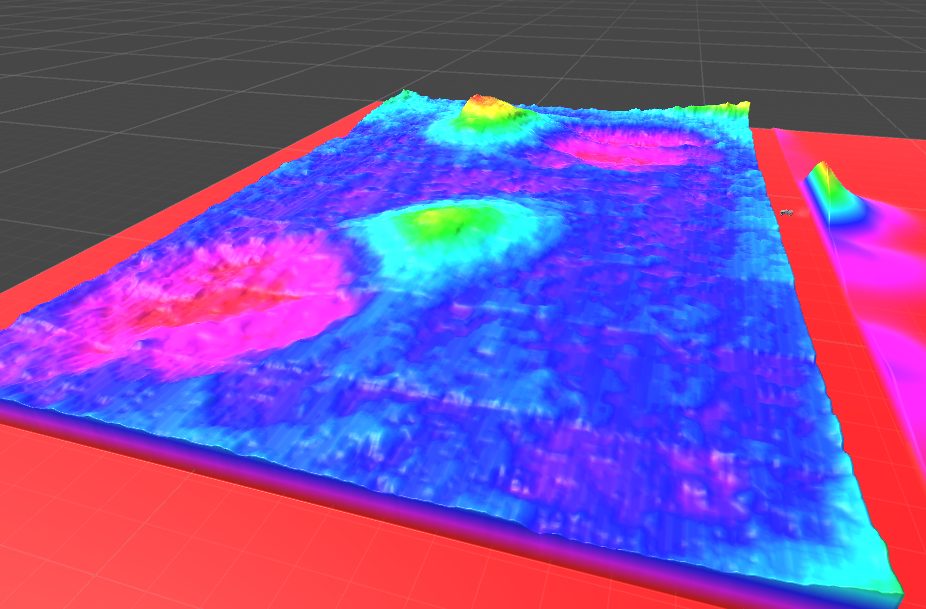
\includegraphics[width=0.8\linewidth]{figures/sandboxHeightShade}
	\caption{Rendered height map on the client using a height color shader}
	\label{fig:sandboxheightshade}
\end{figure}

\subsection{Client}
The client is written in c++ and uses the \textit{Unity} engine. Initially it was planed to use the \textit{Unreal} engine. However, it was not possible to modify terrain at runtime with it. \textit{Unity}, on the other hand, implemented this feature may versions ago. 

\textit{Unreal}s example vehicle implementation was more usable for this scenario since it was a sand buggy and served as inspiration for the project name. But because of the previous mentioned reason \textit{Unity} had to be used and with it its example vehicle implementation. Unfortunately, this was a street car with skid mark animations and screeching sounds. Consequently, the driving performance on the bumpy sand surface was poor. A lift of the car's body and colliders along with an increase in the range of the wheel's suspension improved that performance to acceptable levels. (also see Figure \ref{fig:streetcarbuggy}) There was not enough time/manpower to build proper car physics.   

\begin{figure}
	\centering
	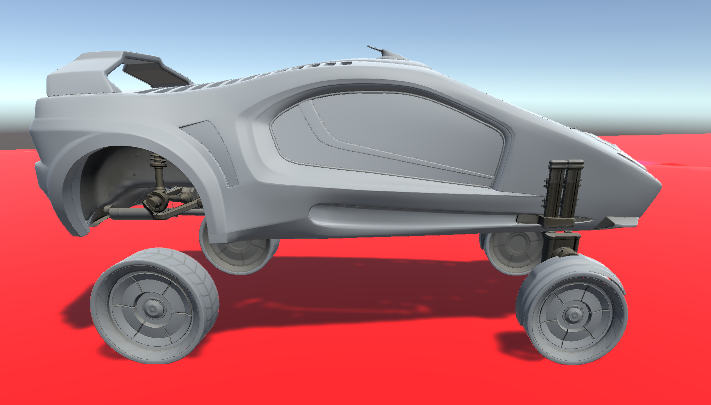
\includegraphics[width=0.7\linewidth]{figures/streetcarbuggy}
	\caption{\textit{Unity}'s demo car adjusted for desert use. The vertical lines in the terrain are an artifact of the sandbox application, possibly cause by the too low resolution of the \textit{Kinnect}.}
	\label{fig:streetcarbuggy}
\end{figure}

To improve the driving experience further the sand terrain was smoothed by a simple median filter. In the same step the region around the car was protected from change. This was done to avoid having an update move the terrain which was under the car above it and causing the car to fall through the map.

Other filters which could be turned on allowed to reduce heights which were at the maximum level and scale the height map to the full range. In the early phases of the project the sand surface was not as pronounced as desired. This was especially true since the base plane offset error (mentioned in the previous chapter) was not discovered. To counter this, I introduced a filter that measured the highest and lowest point in the height map and scaled the map in such a way that those points resided at the highest and lowest point possible of the terrain object. Initially, this worked not as desired since everything that was out of \textit{Magic Sand}'s region of interest was set to the highest value. Reducing those values allowed the rescaling to achieve the desired effect. However, caution needed to applied since setting those values to zero simply would have turned the problem on its head. 

After the offset error was discovered and fixed, those filters were less needed. But still they help to produce more pronounced looking landscapes. Later it turned out that they are unsuited for use in an actual game scenario. During the game the height of the lowest and highest points change constantly and, even worse, sometimes the body parts of the sandbox players are recognized as high height parts of the sand surface thereby the scaling is constantly changing and the rendered surface feels very unstable for the driving player.

\TODO{pictures of (un)scaled/nulled}

For a proof-of-concept back-projection which will be later discussed in chapter \ref{ch:backProjection} a height color shader hat to be implemented. The height of the terrain was used as hue value of a color in the HSL color model. This color was then translated to RGB and used to paint the corresponding point on the terrain texture. An example can be seen in figure \ref{fig:sandboxheightshade}.

To test the game in VR, the VR assets were downloaded from the \textit{Unity Asset Store} and put into the game. They worked without an issue and allowed to take a first glimpse of how a finished game may look. 
 

\subsection{Protocol}
\label{ch:protocol}


too fast -> people are visible in the sand



using two ports was mistake but no time to fix,
maybe not

\subsection{Repositories}
All modules used \textit{git} as version control. The servers are \textit{openframeorks} apps and need to be put in the corresponding folder to work correctly.

\begin{itemize}
	\item The \textit{git} repository of the server can be found at:\\ \url{https://github.com/moreApi/Magic-Sand-Buggy}
	\item The \textit{git} repository of the dummy server can be found at:\\ \url{https://github.com/moreApi/OfServerTest}
	\item The \textit{git} repository of the client can be found at:\\ \url{https://github.com/moreApi/MagicSandBuggyUnity}
\end{itemize}

\section{Discussion}

\subsection{Back-Projection}
\label{ch:backProjection}
streaming unity cam not doable in time
two camera approach - single client
different textures for terrain -> different render runs
streaming camera out of unity to streaming service is hard and not openly done before
two client solution
the whole game was build in single player
not enouth experience to split it in short time

\subsection{Improvements}
Was only a single person

buggy graphic, sprite or drawing instead of dot

smoothing between transitons buggy/sand
only do (big) changes of terrain when not in view

pick ups

car physics

raceing game stuff 


\subsection{Ethical Concerns}
vs. natural interaction (traditional sandbox), tech/advancemend allways good?

racial body issues, handicaped people

more and more technologial playground ->higher entrance borders - body, monetary issues -> more exclusive 


\section{Conclusion}

will continue, at least for feature jam
fun project
will ask pb museum if they want sandbox


% ************************************************************
% *****                      Ende                        *****
% ************************************************************

\end{document}